
\subsection{Non-inverting buck-boost converter\label{N_INV_BB}}
		
The non-inverting buck-boost converter is a DC-DC converter that allows the voltage at its output to be higher or lower than the voltage at its input. The equivalent circuit diagram can be seen in figure \ref{N_INV_BB_SCHEMATIC}. It uses a DC source, 4 switches, of which 2 are controlled devices, two capacitors, an inductor and a load.
		
\begin{figure}[H]
	\begin{center}
	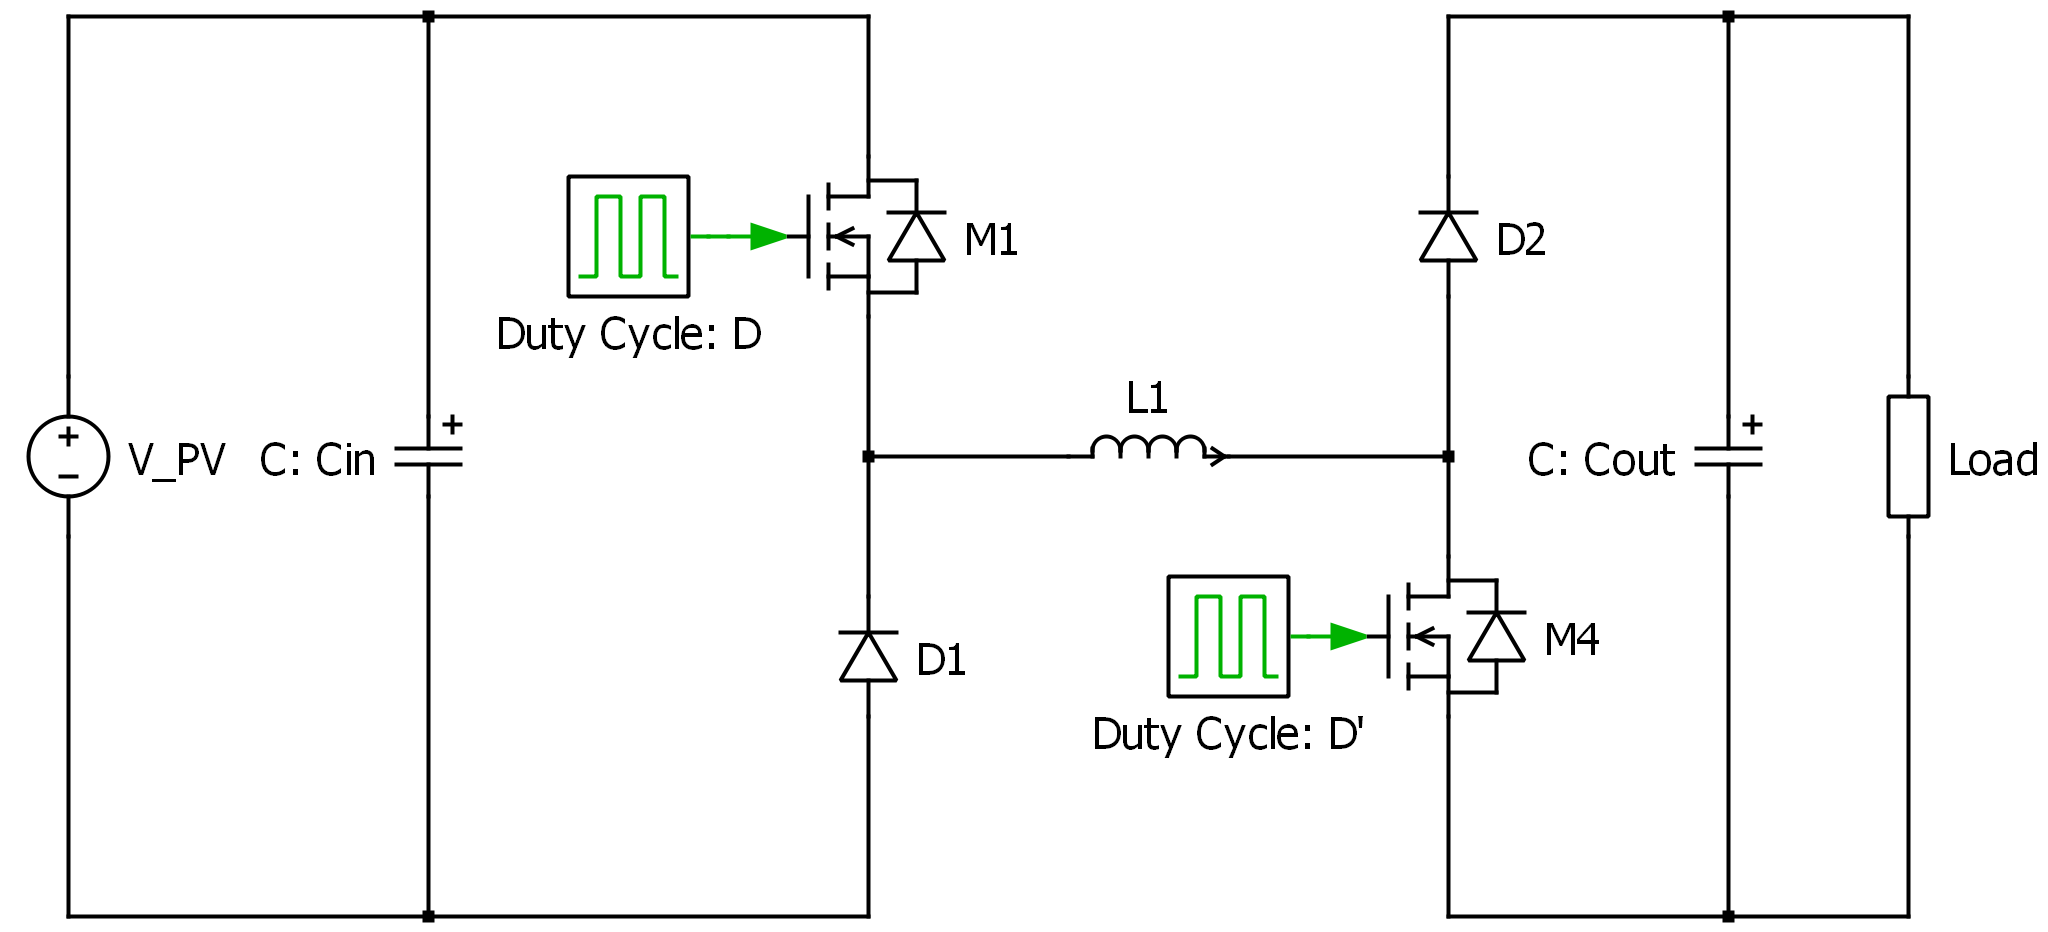
\includegraphics[width=0.8\textwidth]{../Pictures/2_d_H_B_BB}
	\caption{Equivalent circuit for the non-inverting buck-boost converter.}
	\label{N_INV_BB_SCHEMATIC}
	\end{center}	
\end{figure}
	
The controller can force the system to work in any of the following modes:

\begin{enumerate}
	\item Buck $\rightarrow$ $ D \subset [0,1];	 D' = 0 $
	\item Boost $\rightarrow$ $ D = 1;	 D' \subset [0,1] $
	\item Buck-Boost $\rightarrow$ $ D \subset [0,1]; D' \subset [0,1] $
\end{enumerate}
		
Usually, the inverter's input voltage (DC-link voltage) is fixed to some value higher than the peak grid's voltage. The possibility of higher and lower voltages at the converter's output allows different ways of associating photovoltaic modules. Then, the user is able to arbitrarily decide how many PV modules to link in series. Differently of what would happen in the case of buck or boost converters where the constraints regarding the number of panels are a bigger concern \todo{Why? Add reference. Stef}.
		
Compared with other topologies that can have both higher and lower voltages at the output, this DC-DC converter features a single inductor and no intermediate capacitor. With such reduction in passive components the price, efficiency and power density improves significantly \cite{underthehood}. One of the drawbacks of the non-inverting buck-boost topology is the control's complexity, which must calculate the appropriate duty cycle $D$ and $D'$ in any of the modes and also the transition between these modes. The buck-boost mode is specially complicated as there are two duty cycles to calculate. This problem might be addressed by setting a constant duty cycle in one of the bridge's legs and then the control will calculate the other leg's duty cycle  \cite{AN4449_ST}.
		
Although this topology exhibits appropriate features, it can be further improved by replacing the diodes by MOSFETs. The circuit may be seen in figure \ref{BID_N_INV_BB_SCHEMATIC} and it is called Bidirectional Non-Inverting Buck-Boost converter.

\begin{figure}[H]
	\begin{center}
		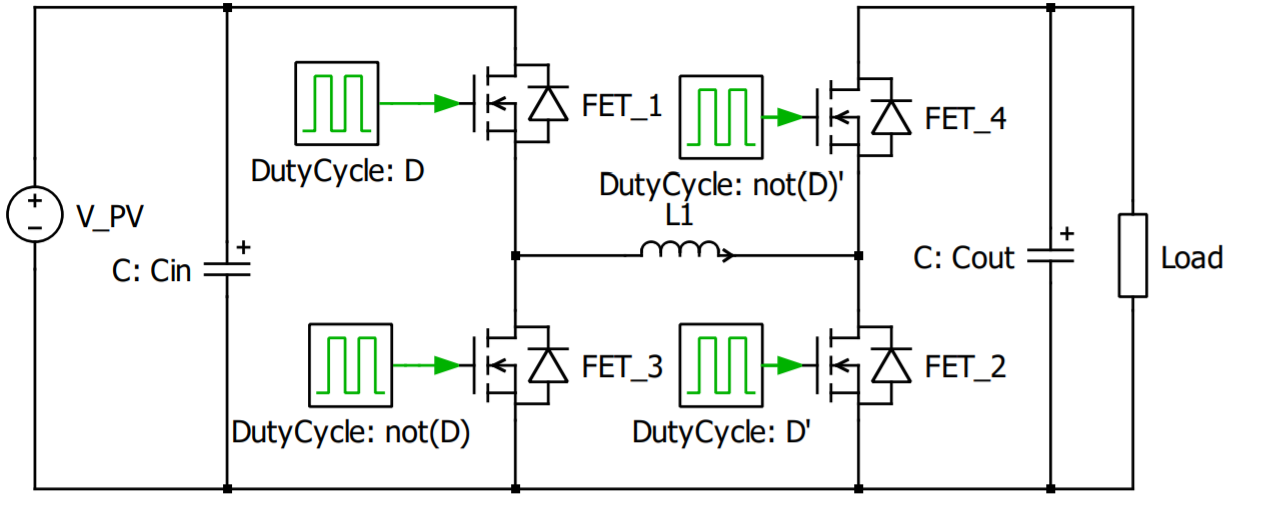
\includegraphics[width=0.8\textwidth]{../Pictures/BID_H_B_BB}
		\caption{Bidirectional Non-inverting buck-boost converter.}
		\label{BID_N_INV_BB_SCHEMATIC}
	\end{center}
\end{figure}

With this variation, the following changes occur:
		
\begin{enumerate}
	\item The system becomes bidirectional.
	\item The conduction losses are smaller. 
\end{enumerate}
\todo{Add reference. Stef}	

If the system is bidirectional it can be used for different purposes, as the topology seen in figure \ref{BID_MIC_ARCHITECTURES}, which features an isolated DC-link. This topology needs a bidirectional MIC as energy flow in both directions is needed. It also allows diagnosis of PV modules \todo{reference. Stef}.

\begin{figure}[H]
	\begin{center}
		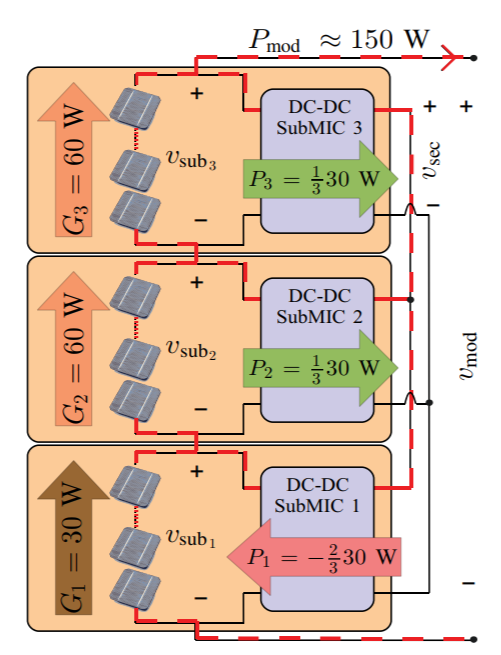
\includegraphics[width=0.4\textwidth]{../Pictures/bidirectional_mic_use}
		\caption{Bidirectional MIC use \cite{ArchitectureMIC}.}
		\label{BID_MIC_ARCHITECTURES}
	\end{center}	
\end{figure}
\todo{I don't know if this figue is necessary as it isn't describe that much.. maybe better just say it with words and delte it or describe better the figure. Stef}		
		
As seen in figure \ref{BID_N_INV_BB_SCHEMATIC}, the duty cycles of the switches that replace the diodes are $\overline{D}$ and $\overline{D'}$. This line over the variables means that it is the complementary value of the original variable. The duty cycle is the boolean variable that indicates the conduction state of a switch. 
		
Another drawback\todo{what is the other drawback? Stef} of the bidirectional system is the increased difficulty of the driver circuitry and the requirement of a dead time in order to avoid the short circuit of $FET_1$ and $FET_3$ or $FET_2$ and $FET_4$, which could damage the system. When using diodes, the system is intrinsically protected against a shoot-through event.\todo{reference. Stef}
		
